\documentclass[main.tex]{subfiles}
\begin{document}

\section{Digital Results}
\subsection{-digitizer description + digitizer output description}

\subsection{-integrating waveforms: QDC spectra}
\begin{figure}[ht]
    \centering
        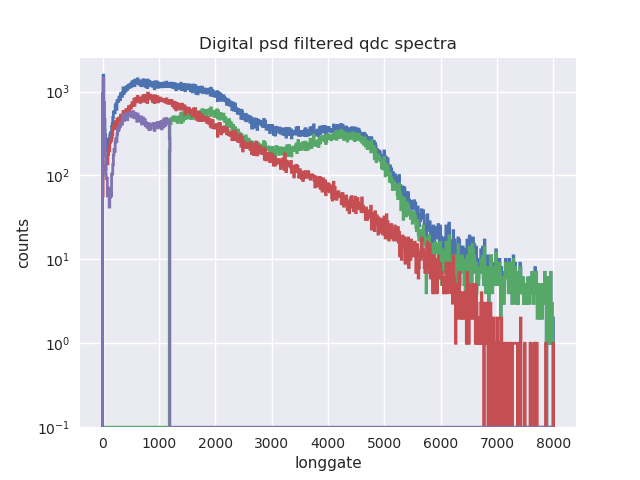
\includegraphics[scale=.75]{DigitalResults/qdc_psd.png}
        \caption{The digital energy spectrum.}
    \label{fig:D_QDC}
\end{figure}

\subsection{PSD}
PSD from longgate and shortgate integration, filtered time of flight.

\begin{figure}
    \centering
    \begin{subfigure}[b]{0.9\textwidth}
        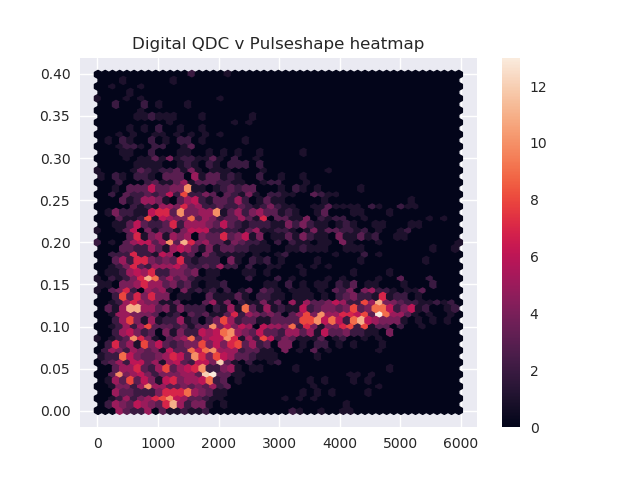
\includegraphics[width=\textwidth]{DigitalResults/psd_hexbin.png}
        \caption{Hexbin heatmap of Pulse shape distribution. The upper band is neutrons and the lower one is gammas.}
        \label{fig:hex_a}
    \end{subfigure}
    \begin{subfigure}[b]{0.9\textwidth}
        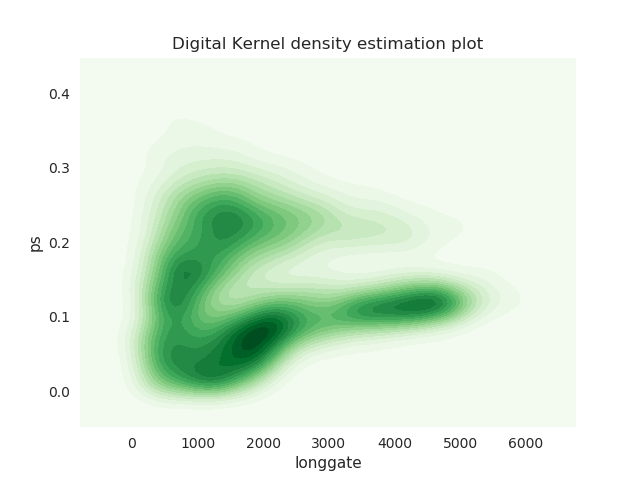
\includegraphics[width=\textwidth]{DigitalResults/psd_kde.png}
        \caption{Kernel density estimation plot of the pulse shape spectrum. The upper band is neutrons and the lower one is gammas.}
        \label{fig:kde_a}
    \end{subfigure}
\label{fig:animals}
\end{figure}

\subsection{-timestamping: cfd: ToF}

The detector signals are led through a patch panel and into an attenuator in order to lower the signal amplitudes. From there they are fed directly into the digitizer. The digitizer will trigger on all enabled channel when the threshold on one channel is surpassed, so a lot of the events will be empty and some will consists of partially contained events. The digitizer used for this project was a a model vx1751 from CAEN, and controlled through the software WaveDumpis. The format of the data is:

\{number of samples per window, digitizer model id, Channel number, Event Number, mask, trigger timestamp, DC offset (DAC), samples\}

%channel mask: decimal representation of the channelmask sent to the digitizer. For an eigth channel digitizer an eigth bit array is sent, with each index setting a channel on or off. $5\rightarrow 00000101\rightarrow$ channel 0 and 1 enabled.

The digitizer triggers on all enabled channels at the same time, so often when a pulse is recorded in one channel nothing an empty sampling window is recorded in the other channels. The data received from the digitizer is processed in order to throw away these empty events, as well as to extract additional features such integrated charge, height, width and a corrected timestamp.

In order to get a good time of flight spectrum we need to have a precise timestamp for each pulse from the detectors. A general timestamp is provided by the digitizer for each event, but a single event may be hundreds or thousands of samples long. For the vc1751 digitizer each sample corresponds to 1 ns, and with detector signals from the NE213 detector and the YAPs ranging from 10-100 ns, then the timestamp needs to be refined.

Fig \ref{fig:not-aligned} shows five pulses from the NE213 detector. The approximate location of the pulses in the sampling window can be specified when the digitizer is configured, through the posttrigger parameter. However, this is not very precise, and the pulses may be located several tens of nanoseconds apart. 

Aligning pulses by peak height location \ref{fig:peak-aligned} results in some improvement but also leads to timewalk.

The leading edge method employed to get \ref{fig:leading_edge-aligned} aligns all pulses around the points where they first surpass a fixed threshold. This method can provide good results provided that the threshold is small compared to the lowest pulseheights. 

By using a constant fraction discrimination (cfd) algorithm the five pulses have been aligned in Fig \ref{fig:cfd-aligned}. The cfd algorithm simply scans through an event and locates the first bin to reach a chosen fraction of the pulse's peak value. In Fig \ref{fig:alignment} 50\% of the peak height was used as the constant fraction. 

Both the leading edge and the cfd algorithm align all the pulses within one nanosecond of each other. Thus by adding the time value acquired by either of these algorithms we get the precision we need in order to perform time of flight measurements.
%INSERT PLOTS

\begin{figure}[ht]
    \centering
        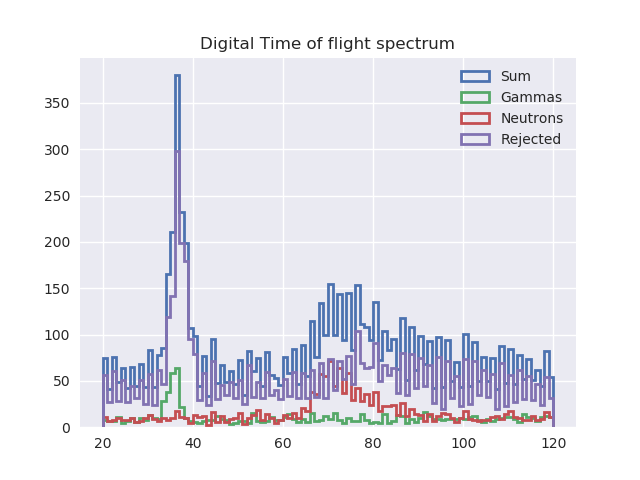
\includegraphics[scale=.75]{DigitalResults/tof_psd.png}
        \caption{The digital time of flight spectrum, filtered using psd classification.}
    \label{fig:D_PSD_TOF} 
\end{figure}

\subsection{Pulse shape v ToF}
\begin{figure}[ht]
    \centering
        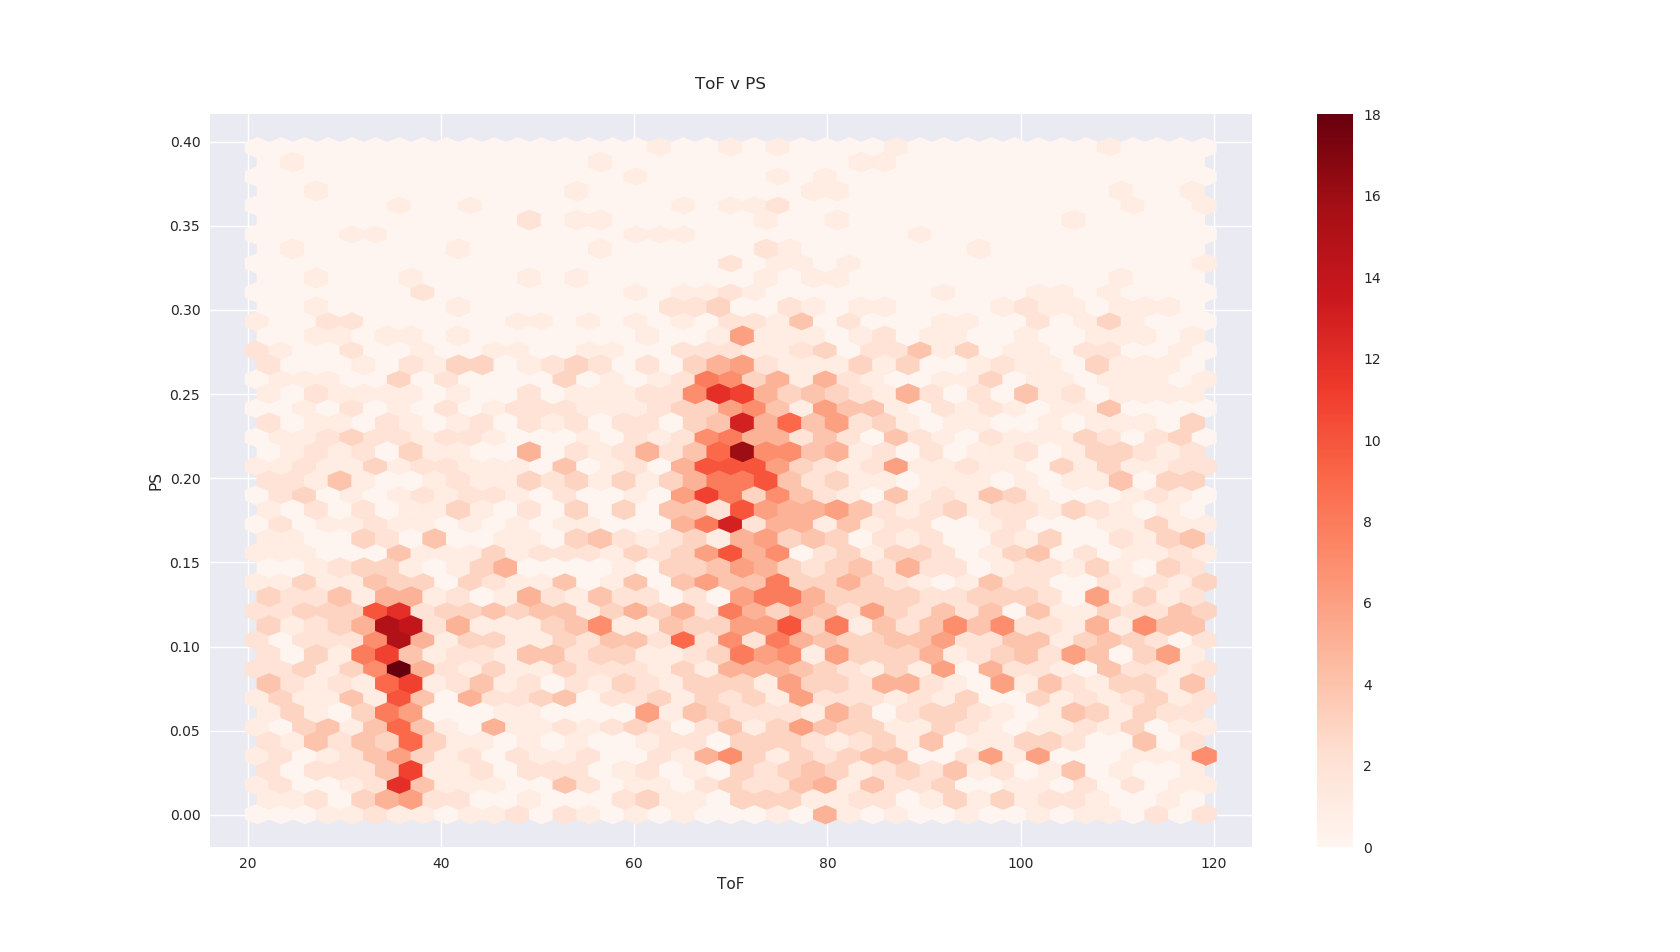
\includegraphics[scale=.35]{DigitalResults/tof_ps_d.png}
        \caption{heatmap of ToF vs pulse shape.}
    \label{fig:tof_ps_d} 
\end{figure}

\end{document}